\documentclass[11pt]{article}
\usepackage[margin=2.5cm]{geometry}
\usepackage[T1]{fontenc}
\usepackage[utf8]{inputenc}
\usepackage{lmodern}
\usepackage{amsmath,amssymb,amsthm}
\usepackage{booktabs}
\usepackage{xcolor}
\usepackage{tikz}
\usepackage{fancyvrb}
\usepackage{newunicodechar}
\usepackage{hyperref}
\hypersetup{colorlinks=true,linkcolor=black,urlcolor=blue,citecolor=black}
\definecolor{cbblue}{HTML}{56B4E9}
\definecolor{cborange}{HTML}{E69F00}
\newunicodechar{ξ}{\ensuremath{\xi}}
\newunicodechar{ℓ}{\ensuremath{\ell}}
\newunicodechar{ℂ}{\ensuremath{\mathbb{C}}}
\newunicodechar{ℕ}{\ensuremath{\mathbb{N}}}
\newunicodechar{→}{\ensuremath{\to}}
\newunicodechar{∀}{\ensuremath{\forall}}
\newunicodechar{∃}{\ensuremath{\exists}}
\newunicodechar{∑}{\ensuremath{\sum}}
\newunicodechar{≤}{\ensuremath{\le}}
\newunicodechar{≠}{\ensuremath{\ne}}
\newunicodechar{∧}{\ensuremath{\wedge}}
\newunicodechar{∈}{\ensuremath{\in}}
\newunicodechar{₃}{\ensuremath{_3}}
\newtheorem{theorem}{Theorem}
\newtheorem{proposition}[theorem]{Proposition}
\newtheorem{corollary}[theorem]{Corollary}
\theoremstyle{remark}
\newtheorem{remark}[theorem]{Remark}
\newcommand{\PAF}{\operatorname{PAF}}
\newcommand{\Z}{\mathbb{Z}}

\title{A ternary Legendre pair of length 35}
\author{Qianghao Wu}
\date{November 25, 2026}

\begin{document}
\emergencystretch=3em
\maketitle

\begin{abstract}
Kotsireas, Liu and Winterhof conjectured that ternary Legendre pairs exist for every length $\ell \equiv -1 \pmod 3$. They found ternary Legendre pairs for every such length $\ell \le 32$ and named $\ell = 35$ and $\ell = 38$ as the smallest open cases. We give a ternary Legendre pair of length 35. This settles the case $\ell = 35$. Both sequences of the pair are invariant under the multiplier $j \mapsto 6j \pmod{35}$. We found the pair with an exact meet-in-the-middle search over the 42\,042\,000 sequences that have this symmetry and the required symbol composition. The search gives 2400 ordered pairs. Lean~4 with Mathlib checks the existence theorem, stated from the source's definition, with kernel evaluation and only the standard axioms. Two exact checkers in Python also accept the pair. The case $\ell = 38$ remains open: our searches in some structured families of length 38 found no pair. This work has not yet been reviewed by experts. The computations, the proofs and the text were produced by AI models (from Anthropic and OpenAI), working under the author's direction.
\end{abstract}

\section{Introduction}

Let $A = [a_0, \dots, a_{\ell-1}] \in \mathbb{C}^\ell$ with $\ell \ge 2$, continued periodically with period $\ell$. Its periodic autocorrelation function at lag $s$ is
\[
  \PAF(A, s) = \sum_{j=0}^{\ell-1} a_j \, \overline{a_{j+s}}, \qquad s = 0, 1, \dots, \ell - 1 .
\]
Two sequences $A$, $B$ of length $\ell$ form a \emph{Legendre pair} if
\begin{equation}\label{eq:lp}
  \PAF(A, s) + \PAF(B, s) = -2, \qquad s = 1, 2, \dots, \lfloor \ell/2 \rfloor .
\end{equation}
Since $\PAF(A, \ell - s) = \overline{\PAF(A, s)}$, condition~\eqref{eq:lp} then holds for all $s = 1, \dots, \ell - 1$. Let $\xi_3 = e^{2\pi\sqrt{-1}/3}$. The pair is \emph{ternary} if $A, B \in \{1, \xi_3, \xi_3^2\}^\ell$. These definitions are those of Kotsireas, Liu and Winterhof~\cite{KLW}, Section~1. We write a ternary sequence as an \emph{exponent word} $r_0 r_1 \cdots r_{\ell-1}$ with $r_j \in \{0, 1, 2\}$, which means $a_j = \xi_3^{r_j}$.

\paragraph{History.} Binary Legendre pairs ($A, B \in \{\pm 1\}^\ell$) give Hadamard matrices of order $2\ell + 2$. Kotsireas, Liu and Winterhof~\cite[Section~1]{KLW} summarize the known infinite families and state that $\ell = 115$ is the smallest undecided binary length. Composite binary lengths are searched with compression and with fixed row and column sums; this method gave the first Legendre pair of length 77~\cite{TKBG}. Recent work on binary pairs studies multipliers: Ramos, Hulak and de~Queiroz~\cite{RHQ} study pairs of length 333 in which both sequences are fixed by a common subgroup $H$ of $(\Z/333\Z)^\times$, and Bulutoglu, Baczkowski and Yauney~\cite{BBY} determine the group of operations that send Legendre pairs to equivalent pairs.

Kotsireas and Winterhof~\cite{KW} introduced quaternary Legendre pairs ($A, B \in \{1, i, -1, -i\}^\ell$), which give quaternary Hadamard matrices of order $2\ell + 2$. Jedwab and Pender~\cite{JP} gave two infinite constructions of even length. According to~\cite[Section~1]{KLW}, Kotsireas, Koutschan and Winterhof~\cite{KW,KKW} found the remaining quaternary pairs of even length $\ell \le 40$. Lebedev~\cite{Leb} found pairs of lengths 42, 46, 52, 58, 66, 72 and 80, and Verma~\cite{Ver} found a pair of length 64.

\paragraph{Ternary pairs.} The source of the question is~\cite{KLW}. Its results for $k$-ary pairs ($A, B \in \{1, \xi_k, \dots, \xi_k^{k-1}\}^\ell$) include:
\begin{itemize}
  \item For prime $k$, a $k$-ary Legendre pair of length $\ell$ exists only if $\ell \equiv -1 \pmod k$~\cite[Theorem~1]{KLW}. For $k = 3$ these lengths are called \emph{admissible}.
  \item For an odd prime $p$, after each component is multiplied by a suitable $p$-th root of unity, the components have a fixed symbol composition~\cite[Theorem~4]{KLW}. For $k = 3$ and $\ell = 3h - 1$, each normalized component contains $1$, $\xi_3$, $\xi_3^2$ exactly $h-1$, $h$, $h$ times~\cite[Section~4]{KLW}.
  \item Every $p$-ary Legendre pair of length $\ell$ gives a Butson Hadamard matrix $H(2p, 2\ell + 2)$~\cite[Corollary~6]{KLW}.
  \item Generalized m-sequences give ternary pairs of every length $3^r - 1$~\cite[Section~2.3]{KLW}.
  \item Searches with fixed-content necklaces, integral-PAF symmetries, half-frequency restrictions, compression and PSD tests give ternary pairs of lengths 5, 11, 14, 17, 20, 23, 29 and 32~\cite[Section~4, Appendix~A]{KLW}. Together with the m-sequence lengths 2, 8 and 26, this covers every admissible $\ell \le 32$.
  \item For $\ell = 38$, the power spectral density $\mathrm{PSD}(C, s) = |\sum_j c_j \xi_{38}^{js}|^2$ at the half frequency leaves three cases, $(\mathrm{PSD}(A,19), \mathrm{PSD}(B,19)) \in \{(3,75), (21,57), (39,39)\}$, up to the exchange of $A$ and $B$~\cite[Section~4.4]{KLW}.
\end{itemize}
The source then states~\cite[Section~1]{KLW}: ``In this way we obtain ternary Legendre pairs for every admissible length $\ell \le 32$. The smallest open cases are then $\ell = 35$ and $\ell = 38$.'' Section~4.4 of~\cite{KLW} states:
\begin{quote}
Conjecture 10. Ternary Legendre pairs exist for every admissible length $\ell \equiv -1 \pmod 3$.
\end{quote}
and ``The next open cases are 35 and 38.''

\paragraph{Result.} We give a ternary Legendre pair of length 35 (Theorem~\ref{thm:main}). So $\ell = 35$ is no longer an open case of Conjecture~10, and the smallest open case is $\ell = 38$. The result does not prove the conjecture.

\paragraph{Prior art.} On November 24 and 25, 2026, we searched arXiv (API queries for ``ternary Legendre'', ``k-ary Legendre'' and ``Legendre pairs'', and the new listings of math.CO and cs.IT), Zenodo, GitHub code and repositories, OEIS, MathOverflow, OpenAlex and the web. We found no other ternary Legendre pair of length 35 or 38. The source appeared on arXiv on November 23, 2026. We cannot exclude unpublished pairs by its authors or by others.

\section{The pair}

\begin{theorem}\label{thm:main}
The sequences with exponent words
\begin{align*}
A &= \texttt{02021220020100021222201110110121211},\\
B &= \texttt{01222010111021021121200221100200122}
\end{align*}
form a ternary Legendre pair of length 35.
\end{theorem}

\begin{figure}[t]
\centering
% Generated by checks/draw_pair.py from data/lp35.txt. Do not edit.
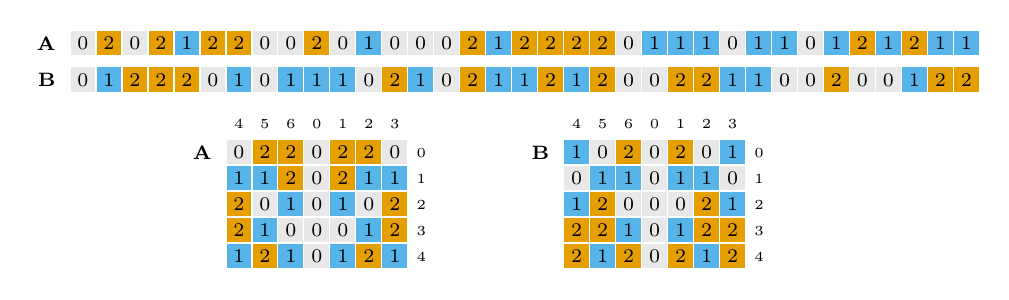
\begin{tikzpicture}[x=3.3mm,y=-3.3mm,every node/.style={font=\scriptsize}]
\node[anchor=east] at (-0.2,0.5) {$\mathbf{A}$};
\fill[black!9] (0,0.0) rectangle +(0.95,0.95); \node at (0.475,0.5) {0};
\fill[cborange] (1,0.0) rectangle +(0.95,0.95); \node at (1.475,0.5) {2};
\fill[black!9] (2,0.0) rectangle +(0.95,0.95); \node at (2.475,0.5) {0};
\fill[cborange] (3,0.0) rectangle +(0.95,0.95); \node at (3.475,0.5) {2};
\fill[cbblue] (4,0.0) rectangle +(0.95,0.95); \node at (4.475,0.5) {1};
\fill[cborange] (5,0.0) rectangle +(0.95,0.95); \node at (5.475,0.5) {2};
\fill[cborange] (6,0.0) rectangle +(0.95,0.95); \node at (6.475,0.5) {2};
\fill[black!9] (7,0.0) rectangle +(0.95,0.95); \node at (7.475,0.5) {0};
\fill[black!9] (8,0.0) rectangle +(0.95,0.95); \node at (8.475,0.5) {0};
\fill[cborange] (9,0.0) rectangle +(0.95,0.95); \node at (9.475,0.5) {2};
\fill[black!9] (10,0.0) rectangle +(0.95,0.95); \node at (10.475,0.5) {0};
\fill[cbblue] (11,0.0) rectangle +(0.95,0.95); \node at (11.475,0.5) {1};
\fill[black!9] (12,0.0) rectangle +(0.95,0.95); \node at (12.475,0.5) {0};
\fill[black!9] (13,0.0) rectangle +(0.95,0.95); \node at (13.475,0.5) {0};
\fill[black!9] (14,0.0) rectangle +(0.95,0.95); \node at (14.475,0.5) {0};
\fill[cborange] (15,0.0) rectangle +(0.95,0.95); \node at (15.475,0.5) {2};
\fill[cbblue] (16,0.0) rectangle +(0.95,0.95); \node at (16.475,0.5) {1};
\fill[cborange] (17,0.0) rectangle +(0.95,0.95); \node at (17.475,0.5) {2};
\fill[cborange] (18,0.0) rectangle +(0.95,0.95); \node at (18.475,0.5) {2};
\fill[cborange] (19,0.0) rectangle +(0.95,0.95); \node at (19.475,0.5) {2};
\fill[cborange] (20,0.0) rectangle +(0.95,0.95); \node at (20.475,0.5) {2};
\fill[black!9] (21,0.0) rectangle +(0.95,0.95); \node at (21.475,0.5) {0};
\fill[cbblue] (22,0.0) rectangle +(0.95,0.95); \node at (22.475,0.5) {1};
\fill[cbblue] (23,0.0) rectangle +(0.95,0.95); \node at (23.475,0.5) {1};
\fill[cbblue] (24,0.0) rectangle +(0.95,0.95); \node at (24.475,0.5) {1};
\fill[black!9] (25,0.0) rectangle +(0.95,0.95); \node at (25.475,0.5) {0};
\fill[cbblue] (26,0.0) rectangle +(0.95,0.95); \node at (26.475,0.5) {1};
\fill[cbblue] (27,0.0) rectangle +(0.95,0.95); \node at (27.475,0.5) {1};
\fill[black!9] (28,0.0) rectangle +(0.95,0.95); \node at (28.475,0.5) {0};
\fill[cbblue] (29,0.0) rectangle +(0.95,0.95); \node at (29.475,0.5) {1};
\fill[cborange] (30,0.0) rectangle +(0.95,0.95); \node at (30.475,0.5) {2};
\fill[cbblue] (31,0.0) rectangle +(0.95,0.95); \node at (31.475,0.5) {1};
\fill[cborange] (32,0.0) rectangle +(0.95,0.95); \node at (32.475,0.5) {2};
\fill[cbblue] (33,0.0) rectangle +(0.95,0.95); \node at (33.475,0.5) {1};
\fill[cbblue] (34,0.0) rectangle +(0.95,0.95); \node at (34.475,0.5) {1};
\node[anchor=east] at (-0.2,1.9) {$\mathbf{B}$};
\fill[black!9] (0,1.4) rectangle +(0.95,0.95); \node at (0.475,1.9) {0};
\fill[cbblue] (1,1.4) rectangle +(0.95,0.95); \node at (1.475,1.9) {1};
\fill[cborange] (2,1.4) rectangle +(0.95,0.95); \node at (2.475,1.9) {2};
\fill[cborange] (3,1.4) rectangle +(0.95,0.95); \node at (3.475,1.9) {2};
\fill[cborange] (4,1.4) rectangle +(0.95,0.95); \node at (4.475,1.9) {2};
\fill[black!9] (5,1.4) rectangle +(0.95,0.95); \node at (5.475,1.9) {0};
\fill[cbblue] (6,1.4) rectangle +(0.95,0.95); \node at (6.475,1.9) {1};
\fill[black!9] (7,1.4) rectangle +(0.95,0.95); \node at (7.475,1.9) {0};
\fill[cbblue] (8,1.4) rectangle +(0.95,0.95); \node at (8.475,1.9) {1};
\fill[cbblue] (9,1.4) rectangle +(0.95,0.95); \node at (9.475,1.9) {1};
\fill[cbblue] (10,1.4) rectangle +(0.95,0.95); \node at (10.475,1.9) {1};
\fill[black!9] (11,1.4) rectangle +(0.95,0.95); \node at (11.475,1.9) {0};
\fill[cborange] (12,1.4) rectangle +(0.95,0.95); \node at (12.475,1.9) {2};
\fill[cbblue] (13,1.4) rectangle +(0.95,0.95); \node at (13.475,1.9) {1};
\fill[black!9] (14,1.4) rectangle +(0.95,0.95); \node at (14.475,1.9) {0};
\fill[cborange] (15,1.4) rectangle +(0.95,0.95); \node at (15.475,1.9) {2};
\fill[cbblue] (16,1.4) rectangle +(0.95,0.95); \node at (16.475,1.9) {1};
\fill[cbblue] (17,1.4) rectangle +(0.95,0.95); \node at (17.475,1.9) {1};
\fill[cborange] (18,1.4) rectangle +(0.95,0.95); \node at (18.475,1.9) {2};
\fill[cbblue] (19,1.4) rectangle +(0.95,0.95); \node at (19.475,1.9) {1};
\fill[cborange] (20,1.4) rectangle +(0.95,0.95); \node at (20.475,1.9) {2};
\fill[black!9] (21,1.4) rectangle +(0.95,0.95); \node at (21.475,1.9) {0};
\fill[black!9] (22,1.4) rectangle +(0.95,0.95); \node at (22.475,1.9) {0};
\fill[cborange] (23,1.4) rectangle +(0.95,0.95); \node at (23.475,1.9) {2};
\fill[cborange] (24,1.4) rectangle +(0.95,0.95); \node at (24.475,1.9) {2};
\fill[cbblue] (25,1.4) rectangle +(0.95,0.95); \node at (25.475,1.9) {1};
\fill[cbblue] (26,1.4) rectangle +(0.95,0.95); \node at (26.475,1.9) {1};
\fill[black!9] (27,1.4) rectangle +(0.95,0.95); \node at (27.475,1.9) {0};
\fill[black!9] (28,1.4) rectangle +(0.95,0.95); \node at (28.475,1.9) {0};
\fill[cborange] (29,1.4) rectangle +(0.95,0.95); \node at (29.475,1.9) {2};
\fill[black!9] (30,1.4) rectangle +(0.95,0.95); \node at (30.475,1.9) {0};
\fill[black!9] (31,1.4) rectangle +(0.95,0.95); \node at (31.475,1.9) {0};
\fill[cbblue] (32,1.4) rectangle +(0.95,0.95); \node at (32.475,1.9) {1};
\fill[cborange] (33,1.4) rectangle +(0.95,0.95); \node at (33.475,1.9) {2};
\fill[cborange] (34,1.4) rectangle +(0.95,0.95); \node at (34.475,1.9) {2};
\node[anchor=east] at (5.8,4.7) {$\mathbf{A}$};
\node at (6.475,3.6) {\tiny 4};
\node at (7.475,3.6) {\tiny 5};
\node at (8.475,3.6) {\tiny 6};
\node at (9.475,3.6) {\tiny 0};
\node at (10.475,3.6) {\tiny 1};
\node at (11.475,3.6) {\tiny 2};
\node at (12.475,3.6) {\tiny 3};
\node at (13.5,4.7) {\tiny 0};
\fill[black!9] (6,4.2) rectangle +(0.95,0.95); \node at (6.475,4.7) {0};
\fill[cborange] (7,4.2) rectangle +(0.95,0.95); \node at (7.475,4.7) {2};
\fill[cborange] (8,4.2) rectangle +(0.95,0.95); \node at (8.475,4.7) {2};
\fill[black!9] (9,4.2) rectangle +(0.95,0.95); \node at (9.475,4.7) {0};
\fill[cborange] (10,4.2) rectangle +(0.95,0.95); \node at (10.475,4.7) {2};
\fill[cborange] (11,4.2) rectangle +(0.95,0.95); \node at (11.475,4.7) {2};
\fill[black!9] (12,4.2) rectangle +(0.95,0.95); \node at (12.475,4.7) {0};
\node at (13.5,5.7) {\tiny 1};
\fill[cbblue] (6,5.2) rectangle +(0.95,0.95); \node at (6.475,5.7) {1};
\fill[cbblue] (7,5.2) rectangle +(0.95,0.95); \node at (7.475,5.7) {1};
\fill[cborange] (8,5.2) rectangle +(0.95,0.95); \node at (8.475,5.7) {2};
\fill[black!9] (9,5.2) rectangle +(0.95,0.95); \node at (9.475,5.7) {0};
\fill[cborange] (10,5.2) rectangle +(0.95,0.95); \node at (10.475,5.7) {2};
\fill[cbblue] (11,5.2) rectangle +(0.95,0.95); \node at (11.475,5.7) {1};
\fill[cbblue] (12,5.2) rectangle +(0.95,0.95); \node at (12.475,5.7) {1};
\node at (13.5,6.7) {\tiny 2};
\fill[cborange] (6,6.2) rectangle +(0.95,0.95); \node at (6.475,6.7) {2};
\fill[black!9] (7,6.2) rectangle +(0.95,0.95); \node at (7.475,6.7) {0};
\fill[cbblue] (8,6.2) rectangle +(0.95,0.95); \node at (8.475,6.7) {1};
\fill[black!9] (9,6.2) rectangle +(0.95,0.95); \node at (9.475,6.7) {0};
\fill[cbblue] (10,6.2) rectangle +(0.95,0.95); \node at (10.475,6.7) {1};
\fill[black!9] (11,6.2) rectangle +(0.95,0.95); \node at (11.475,6.7) {0};
\fill[cborange] (12,6.2) rectangle +(0.95,0.95); \node at (12.475,6.7) {2};
\node at (13.5,7.7) {\tiny 3};
\fill[cborange] (6,7.2) rectangle +(0.95,0.95); \node at (6.475,7.7) {2};
\fill[cbblue] (7,7.2) rectangle +(0.95,0.95); \node at (7.475,7.7) {1};
\fill[black!9] (8,7.2) rectangle +(0.95,0.95); \node at (8.475,7.7) {0};
\fill[black!9] (9,7.2) rectangle +(0.95,0.95); \node at (9.475,7.7) {0};
\fill[black!9] (10,7.2) rectangle +(0.95,0.95); \node at (10.475,7.7) {0};
\fill[cbblue] (11,7.2) rectangle +(0.95,0.95); \node at (11.475,7.7) {1};
\fill[cborange] (12,7.2) rectangle +(0.95,0.95); \node at (12.475,7.7) {2};
\node at (13.5,8.7) {\tiny 4};
\fill[cbblue] (6,8.2) rectangle +(0.95,0.95); \node at (6.475,8.7) {1};
\fill[cborange] (7,8.2) rectangle +(0.95,0.95); \node at (7.475,8.7) {2};
\fill[cbblue] (8,8.2) rectangle +(0.95,0.95); \node at (8.475,8.7) {1};
\fill[black!9] (9,8.2) rectangle +(0.95,0.95); \node at (9.475,8.7) {0};
\fill[cbblue] (10,8.2) rectangle +(0.95,0.95); \node at (10.475,8.7) {1};
\fill[cborange] (11,8.2) rectangle +(0.95,0.95); \node at (11.475,8.7) {2};
\fill[cbblue] (12,8.2) rectangle +(0.95,0.95); \node at (12.475,8.7) {1};
\node[anchor=east] at (18.8,4.7) {$\mathbf{B}$};
\node at (19.475,3.6) {\tiny 4};
\node at (20.475,3.6) {\tiny 5};
\node at (21.475,3.6) {\tiny 6};
\node at (22.475,3.6) {\tiny 0};
\node at (23.475,3.6) {\tiny 1};
\node at (24.475,3.6) {\tiny 2};
\node at (25.475,3.6) {\tiny 3};
\node at (26.5,4.7) {\tiny 0};
\fill[cbblue] (19,4.2) rectangle +(0.95,0.95); \node at (19.475,4.7) {1};
\fill[black!9] (20,4.2) rectangle +(0.95,0.95); \node at (20.475,4.7) {0};
\fill[cborange] (21,4.2) rectangle +(0.95,0.95); \node at (21.475,4.7) {2};
\fill[black!9] (22,4.2) rectangle +(0.95,0.95); \node at (22.475,4.7) {0};
\fill[cborange] (23,4.2) rectangle +(0.95,0.95); \node at (23.475,4.7) {2};
\fill[black!9] (24,4.2) rectangle +(0.95,0.95); \node at (24.475,4.7) {0};
\fill[cbblue] (25,4.2) rectangle +(0.95,0.95); \node at (25.475,4.7) {1};
\node at (26.5,5.7) {\tiny 1};
\fill[black!9] (19,5.2) rectangle +(0.95,0.95); \node at (19.475,5.7) {0};
\fill[cbblue] (20,5.2) rectangle +(0.95,0.95); \node at (20.475,5.7) {1};
\fill[cbblue] (21,5.2) rectangle +(0.95,0.95); \node at (21.475,5.7) {1};
\fill[black!9] (22,5.2) rectangle +(0.95,0.95); \node at (22.475,5.7) {0};
\fill[cbblue] (23,5.2) rectangle +(0.95,0.95); \node at (23.475,5.7) {1};
\fill[cbblue] (24,5.2) rectangle +(0.95,0.95); \node at (24.475,5.7) {1};
\fill[black!9] (25,5.2) rectangle +(0.95,0.95); \node at (25.475,5.7) {0};
\node at (26.5,6.7) {\tiny 2};
\fill[cbblue] (19,6.2) rectangle +(0.95,0.95); \node at (19.475,6.7) {1};
\fill[cborange] (20,6.2) rectangle +(0.95,0.95); \node at (20.475,6.7) {2};
\fill[black!9] (21,6.2) rectangle +(0.95,0.95); \node at (21.475,6.7) {0};
\fill[black!9] (22,6.2) rectangle +(0.95,0.95); \node at (22.475,6.7) {0};
\fill[black!9] (23,6.2) rectangle +(0.95,0.95); \node at (23.475,6.7) {0};
\fill[cborange] (24,6.2) rectangle +(0.95,0.95); \node at (24.475,6.7) {2};
\fill[cbblue] (25,6.2) rectangle +(0.95,0.95); \node at (25.475,6.7) {1};
\node at (26.5,7.7) {\tiny 3};
\fill[cborange] (19,7.2) rectangle +(0.95,0.95); \node at (19.475,7.7) {2};
\fill[cborange] (20,7.2) rectangle +(0.95,0.95); \node at (20.475,7.7) {2};
\fill[cbblue] (21,7.2) rectangle +(0.95,0.95); \node at (21.475,7.7) {1};
\fill[black!9] (22,7.2) rectangle +(0.95,0.95); \node at (22.475,7.7) {0};
\fill[cbblue] (23,7.2) rectangle +(0.95,0.95); \node at (23.475,7.7) {1};
\fill[cborange] (24,7.2) rectangle +(0.95,0.95); \node at (24.475,7.7) {2};
\fill[cborange] (25,7.2) rectangle +(0.95,0.95); \node at (25.475,7.7) {2};
\node at (26.5,8.7) {\tiny 4};
\fill[cborange] (19,8.2) rectangle +(0.95,0.95); \node at (19.475,8.7) {2};
\fill[cbblue] (20,8.2) rectangle +(0.95,0.95); \node at (20.475,8.7) {1};
\fill[cborange] (21,8.2) rectangle +(0.95,0.95); \node at (21.475,8.7) {2};
\fill[black!9] (22,8.2) rectangle +(0.95,0.95); \node at (22.475,8.7) {0};
\fill[cborange] (23,8.2) rectangle +(0.95,0.95); \node at (23.475,8.7) {2};
\fill[cbblue] (24,8.2) rectangle +(0.95,0.95); \node at (24.475,8.7) {1};
\fill[cborange] (25,8.2) rectangle +(0.95,0.95); \node at (25.475,8.7) {2};
\end{tikzpicture}

\caption{The pair of Theorem~\ref{thm:main}. Top: the exponent words, $j = 0, \dots, 34$ from left to right. Bottom: entry $j$ placed in row $j \bmod 5$ and in the column of $j \bmod 7$, with the columns in the order $4, 5, 6, 0, 1, 2, 3$. Since $6j \equiv j \pmod 5$ and $6j \equiv -j \pmod 7$, invariance under $j \mapsto 6j$ makes each row read the same in both directions. The figure is drawn from the certificate by \texttt{checks/draw\_pair.py}.}
\label{fig:pair}
\end{figure}

\begin{proof}
Let $e$ be an exponent word and $a_j = \xi_3^{e_j}$. Since $\overline{\xi_3} = \xi_3^2$ and $\xi_3^3 = 1$, we have $a_j \overline{a_{j+s}} = \xi_3^{(e_j - e_{j+s}) \bmod 3}$. For a lag $s$ and $r \in \{0, 1, 2\}$, let $M_r(s)$ be the number of $j \in \Z/35\Z$ with $(e_j - e_{j+s}) \bmod 3 = r$, counted for $A$ and for $B$ together. Then
\[
  \PAF(A, s) + \PAF(B, s) = M_0(s) + M_1(s)\,\xi_3 + M_2(s)\,\xi_3^2 .
\]
Direct counting gives $(M_0, M_1, M_2)(s) = (22, 24, 24)$ for every $s = 1, \dots, 34$. Since $1 + \xi_3 + \xi_3^2 = 0$, the sum is $22 + 24(\xi_3 + \xi_3^2) = 22 - 24 = -2$.
\end{proof}

This count is the integer test of~\cite[Appendix~A]{KLW}: with $\ell = 3h - 1$, a ternary pair satisfies $(M_0, M_1, M_2)(s) = (2h - 2, 2h, 2h)$, and here $h = 12$. The proof needs the counts only for $s = 1, \dots, 17$; the counts hold for all 34 nonzero lags.

Further facts about the pair, all checked by \texttt{checks/check.py}:
\begin{itemize}
  \item Each word has 11 zeros, 12 ones and 12 twos, that is, composition $(11, 12, 12)$. This agrees with the normalized composition $(h-1, h, h)$ of~\cite{KLW}. Each component has sum $11 + 12\xi_3 + 12\xi_3^2 = -1$.
  \item Both words are invariant under $j \mapsto 6j \pmod{35}$, that is, $e_{6j} = e_j$ for all $j$. The group $\{1, 6\}$ has order 2 and does not contain $-1$. Neither word is invariant under $j \mapsto -j$.
  \item In both words, the entries at the multiples of 7 (the points fixed by $j \mapsto 6j$) are all 0 (Figure~\ref{fig:pair}, middle column of each grid).
\end{itemize}

\begin{remark}
By~\cite[Corollary~6]{KLW}, the pair gives a Butson Hadamard matrix $H(6, 72)$. We did not construct this matrix. We make no claim that an $H(6, 72)$ is new.
\end{remark}

\section{How the pair was found}\label{sec:search}

\paragraph{Multiplier orbits.} Let $H$ be a subgroup of the unit group $\Z_{35}^\times$. A sequence $A$ is \emph{$H$-invariant} if $a_{tj} = a_j$ for all $t \in H$ and all $j$. An $H$-invariant sequence is constant on each orbit of $H$ on $\Z/35\Z$. If $A$ is $H$-invariant and $t \in H$, the substitution $j \mapsto tj$ gives $\PAF(A, ts) = \PAF(A, s)$. The same idea, for binary pairs of length 333, is the subject of~\cite{RHQ}.

For $H = \langle 6 \rangle = \{1, 6\}$, the orbits are the 5 fixed points $0, 7, 14, 21, 28$ and 15 orbits $\{j, 6j\}$ of size 2. So an $H$-invariant word is given by 20 symbols. Exactly 42\,042\,000 of these words have composition $(11, 12, 12)$.

\paragraph{Normalization.} Multiplication of $A$ by a constant $\xi_3^c$ does not change $\PAF(A, s)$, and it keeps $H$-invariance. By~\cite[Theorem~4]{KLW}, every ternary pair of length 35 becomes, after such multiplications of $A$ and of $B$, a pair in which both words have composition $(11, 12, 12)$. So a search over the words with this composition finds an $H$-invariant pair if one exists.

\paragraph{Meet in the middle.} For a fixed $H$, the program \texttt{checks/search/mitm.c} does these steps:
\begin{enumerate}
  \item It lists every $H$-invariant word with composition $(11, 12, 12)$.
  \item For each word $X$ and each lag $s = 1, \dots, 17$, it computes $\PAF(X, s) = u_s + v_s \xi_3$ exactly, with $u_s = N_0(s) - N_2(s)$ and $v_s = N_1(s) - N_2(s)$, where $N_r(s)$ counts the $j$ with $(x_j - x_{j+s}) \bmod 3 = r$. It stores a 64-bit hash of the vector $(u_s, v_s)_{s=1}^{17}$ with the word, and sorts the records by hash.
  \item For each word $A$, it looks up the hash of the target vector $(-2 - u_s, -v_s)_{s=1}^{17}$. For each word $B$ with that hash, it checks $\PAF(A,s) + \PAF(B,s) = -2$ for $s = 1, \dots, 17$ exactly, in integers.
\end{enumerate}
A true pair always has equal hashes, so the hash causes no missed pairs. Each reported pair passed the exact check of step~3. The program counts ordered pairs $(A, B)$.

\paragraph{Results.} Table~\ref{tab:search} gives the runs at $\ell = 35$. Each run used one thread on an Apple M1 Pro. The run for $\langle 6 \rangle$ took about 85\,s. The pair of Theorem~\ref{thm:main} is one of the 2400 pairs that it prints. The 2400 ordered pairs include pairs that are equivalent under shifts, multipliers, conjugation and the exchange of $A$ and $B$. We did not count the equivalence classes.

\begin{table}[t]
\centering
\begin{tabular}{lrrr}
\toprule
$H$ & $|H|$ & $H$-invariant words with composition $(11,12,12)$ & ordered pairs \\
\midrule
$\langle 34\rangle = \{\pm 1\}$ & 2 & 5\,717\,712 & 0 \\
$\langle 6\rangle$ & 2 & 42\,042\,000 & 2400 \\
$\langle 29\rangle$ & 2 & 130\,162\,032 & 0 \\
$\langle 11\rangle$ & 3 & 87\,150 & 0 \\
$\langle 8\rangle$ & 4 & 14\,840 & 0 \\
$\langle 13\rangle$ & 4 & 1\,400 & 0 \\
$\langle 3\rangle$ & 12 & 2 & 0 \\
\bottomrule
\end{tabular}
\caption{Searches at $\ell = 35$: the number of ordered pairs $(A, B)$ in which both $A$ and $B$ are $H$-invariant and have composition $(11, 12, 12)$. The rerun command is \texttt{python3 -I checks/search.py}.}
\label{tab:search}
\end{table}

The group $\Z_{35}^\times$ has 15 subgroups other than $\{1\}$. A direct enumeration (\texttt{checks/check.py}) shows that each of them contains one of the four subgroups of prime order, $\langle 34\rangle$, $\langle 6\rangle$, $\langle 29\rangle$ and $\langle 11\rangle$. If $H \subseteq H'$, every $H'$-invariant word is $H$-invariant. With the zero rows of Table~\ref{tab:search} for $\langle 34\rangle$, $\langle 29\rangle$ and $\langle 11\rangle$, this gives:

\begin{proposition}[computer-assisted]\label{prop:only6}
Let $H \ne \{1\}$ be a subgroup of $\Z_{35}^\times$. A ternary Legendre pair of length 35 in which both components are $H$-invariant exists if and only if $H = \langle 6 \rangle$.
\end{proposition}

The ``only if'' part rests on the search program, which is not formally verified. The ``if'' part is Theorem~\ref{thm:main}. The element 6 acts as $+1$ on $\Z/5\Z$ and as $-1$ on $\Z/7\Z$. We do not have an explanation of why this group gives pairs and the other groups do not.

\section{Verification}

\paragraph{Lean.} The file \texttt{lean/TernaryLP35.lean} imports only Mathlib. It states the definition of~\cite{KLW} over $\mathbb{C}$ and proves the existence theorem:
\begin{Verbatim}[fontsize=\small]
def ξ3 : ℂ := Complex.exp (2 * Real.pi * Complex.I / 3)

def PAF {ℓ : ℕ} [NeZero ℓ] (a : Fin ℓ → ℂ) (s : Fin ℓ) : ℂ :=
  ∑ j : Fin ℓ, a j * (starRingEnd ℂ) (a (j + s))

def IsTernaryLegendrePair (ℓ : ℕ) [NeZero ℓ] (A B : Fin ℓ → ℂ) : Prop :=
  (∀ j, A j ∈ ({1, ξ3, ξ3 ^ 2} : Set ℂ)) ∧
  (∀ j, B j ∈ ({1, ξ3, ξ3 ^ 2} : Set ℂ)) ∧
  ∀ s : Fin ℓ, 1 ≤ s.val → s.val ≤ ℓ / 2 → PAF A s + PAF B s = -2

theorem exists_ternary_legendre_pair_35 :
    ∃ A B : Fin 35 → ℂ, IsTernaryLegendrePair 35 A B
\end{Verbatim}
The definitions match the source line by line:
\begin{itemize}
  \item \texttt{ξ3} is $e^{2\pi\sqrt{-1}/3}$. The proof gets from Mathlib that it is a primitive cube root of unity.
  \item Addition in \texttt{Fin ℓ} is addition modulo $\ell$, so \texttt{a (j + s)} is the periodic continuation $a_{(j+s) \bmod \ell}$. The sum runs over all $\ell$ indices. \texttt{starRingEnd ℂ} is complex conjugation, and it is on the second factor, as in the source.
  \item The lags are $1 \le s \le \ell / 2$, where \texttt{ℓ / 2} is division in $\mathbb{N}$, that is, $\lfloor \ell / 2 \rfloor$. For $\ell = 35$ these are $s = 1, \dots, 17$.
  \item Every entry of $A$ and of $B$ is in $\{1, \xi_3, \xi_3^2\}$: this is the ternary case $k = 3$.
  \item \texttt{[NeZero ℓ]} only makes the arithmetic of \texttt{Fin ℓ} available. It adds no condition for $\ell = 35$.
\end{itemize}
The proof follows the proof of Theorem~\ref{thm:main}. The witnesses are $a_j = \xi_3^{e_j}$ for the two exponent words. A lemma rewrites $\PAF$ as $M_0 + M_1 \xi_3 + M_2 \xi_3^2$. The lemma \texttt{counts\_ok} states that the combined counts are $(22, 24, 24)$ at every nonzero lag, and the kernel proves it with \texttt{decide}. A final \texttt{linear\_combination} with $1 + \xi_3 + \xi_3^2 = 0$ closes the goal. The proof does not use \texttt{native\_decide}. The command \texttt{\#print axioms exists\_ternary\_legendre\_pair\_35} prints
\begin{Verbatim}[fontsize=\footnotesize]
'exists_ternary_legendre_pair_35' depends on axioms: [propext, Classical.choice, Quot.sound]
\end{Verbatim}
These are the standard axioms of Lean and Mathlib; \texttt{Lean.ofReduceBool} does not occur. The file contains no \texttt{sorry}, \texttt{admit}, \texttt{axiom}, \texttt{implemented\_by} or \texttt{unsafe}. With Lean v4.36.0 and Mathlib v4.36.0, the check takes about 1 to 3 minutes on an M1 Pro; three measured runs took 151\,s, 60\,s and 56\,s. In two mutation tests, one entry of the certificate in a copy of the file was changed; each time, \texttt{decide} reported that \texttt{counts\_ok} is false.

\paragraph{Python.} Two exact checkers were written separately. \texttt{checks/check\_pair.py} computes the integer counts $M_r(s)$ for $s = 1, \dots, 34$. \texttt{checks/check\_pair\_zw.py} multiplies in $\Z[\omega] = \Z[x]/(x^2 + x + 1)$ and also reports a floating-point cross-check (maximum error $7.3 \cdot 10^{-15}$). Both accept the pair. Both accept the eight pairs printed in~\cite{KLW} (lengths 5, 11, 14, 17, 20, 23, 29, 32). Both reject each of the 140 pairs that differ from ours in one entry. \texttt{checks/check.py} runs all of these checks in less than 1\,s. It also checks that the words in the Lean file equal the certificate \texttt{data/lp35.txt}.

\paragraph{Independent review.} A second AI session, separate from the session that found the pair, reran the checks from a clean copy. It wrote its own checker (now \texttt{checks/check\_pair\_zw.py}) before it read the first checker. It compared the Lean statement with the source, reran the Lean proof and the searches of Table~\ref{tab:search}, and added the $\langle 29\rangle$ row.

\section{The case \texorpdfstring{$\ell = 38$}{l = 38}}\label{sec:38}

We applied the same exact meet-in-the-middle method at $\ell = 38$, where the normalized composition is $(12, 13, 13)$ and the combined counts must be $(24, 26, 26)$. A family is the set of words $e$ with composition $(12, 13, 13)$ that satisfy $e_{hx + c} \equiv \sigma e_x + k \pmod 3$ for all $x$, for one fixed map $(h, c, \sigma, k)$ with $\sigma = \pm 1$. The sign $\sigma = -1$ means complex conjugation. For example, $(37, 0, 1, 0)$ is the family of symmetric words ($a_{-x} = a_x$), and $(1, 19, -1, 0)$ is the family with $a_{x+19} = \overline{a_x}$. The searched combinations were:
\begin{itemize}
  \item 10 families with themselves: $(27,0,1,0)$ and $(31,0,1,0)$ (180 words each); $(7,1,-1,0)$, $(11,1,-1,0)$, $(27,1,-1,0)$, $(31,1,-1,0)$ (480 each); $(7,0,1,0)$, $(11,0,1,0)$ (69\,300 each); $(37,0,1,0)$ (34\,306\,272); $(37,0,-1,0)$ (70\,189\,056);
  \item 12 combinations of two different families, with family sizes up to 222\,265\,344 (for $(37,1,-1,0)$ and $(1,19,-1,0)$);
  \item $(1,19,-1,0)$ with itself (222\,265\,344 words, run in 5 parts).
\end{itemize}
In total these are 27 runs. All of them found no pair. The full list of runs, with their set sizes, is in \texttt{NUMBERS.md}. The independent review reran 19 of these 27 runs with identical output: the 9 self-runs of the families other than $(37,0,1,0)$, and 10 of the 12 combinations of two different families. For this paper we reran $(37,0,1,0)$ with itself and again found 34\,306\,272 words and 0 pairs. The other 7 runs ($(37,0,1,0)$ with $(37,1,-1,0)$, $(37,0,1,0)$ with $(1,19,-1,0)$, and the 5 parts of $(1,19,-1,0)$ with itself) were not rerun. Each of them holds a set of 222\,265\,344 records, about 3.6\,GB, which is near the 4\,GB memory limit of one job on our machine. These are negative results inside the listed families only. They say nothing about whether a ternary Legendre pair of length 38 exists. A natural next step is the compression method of~\cite{KLW}, run separately in each of the three half-frequency cases; we did not try it.

\section{Limits}
\begin{itemize}
  \item The result settles $\ell = 35$ only. It does not prove Conjecture~10, and $\ell = 38$ remains open.
  \item Theorem~\ref{thm:main} is checked in Lean from the definitions. Proposition~\ref{prop:only6}, the count 2400 and all results at $\ell = 38$ come from a C program that is not formally verified. We make no claim about the number of pairs, or of equivalence classes, of length 35.
  \item The Lean proof uses kernel \texttt{decide} on a statement about 34 lags and two words of length 35. Its run time varies from about 1 to about 3 minutes.
\end{itemize}

\section*{Code and data}
The certificate, the Lean file, the checkers, the search program and the figure script are in the result folder. \texttt{bash checks/ci.sh} reruns all checks and all searches of Table~\ref{tab:search}, and fails if a number differs from this paper.

\begin{thebibliography}{99}
\bibitem{BBY} D.~Bulutoglu, D.~Baczkowski, J.~Yauney, Determining the group that sends each Legendre pair to an equivalent Legendre pair, arXiv:2604.22423 (2026). \url{https://arxiv.org/abs/2604.22423}
\bibitem{JP} J.~Jedwab, T.~Pender, Two constructions of quaternary Legendre pairs of even length, Comb.\ Theory 5 (2025), no.~2, Paper No.~15. arXiv:2408.08472. \url{https://arxiv.org/abs/2408.08472}
\bibitem{KKW} I.~S. Kotsireas, C.~Koutschan, A.~Winterhof, Quaternary Legendre pairs II, Discrete Math.\ 348 (2025), no.~9, Paper No.~114501. arXiv:2408.16318. \url{https://arxiv.org/abs/2408.16318}
\bibitem{KLW} I.~S. Kotsireas, H.~Liu, A.~Winterhof, $k$-ary Legendre pairs, arXiv:2611.31067v1 (November 23, 2026). \url{https://arxiv.org/abs/2611.31067}
\bibitem{KW} I.~S. Kotsireas, A.~Winterhof, Quaternary Legendre pairs, in: New Advances in Designs, Codes and Cryptography, Fields Inst.\ Commun.\ 86, Springer, 2024, pp.~289--304. arXiv:2212.10953. \url{https://arxiv.org/abs/2212.10953}
\bibitem{Leb} N.~Lebedev, Quaternary Legendre pairs of lengths 42, 46, 52, 58, 66, 72, and 80, arXiv:2609.04589 (2026). \url{https://arxiv.org/abs/2609.04589}
\bibitem{Mathlib} The mathlib Community, Mathlib, tag v4.36.0. \url{https://github.com/leanprover-community/mathlib4}
\bibitem{RHQ} A.~F. Ramos, D.~B. Hulak, R.~J.~G.~B. de~Queiroz, Multiplier obstructions for Legendre pairs of length 333, arXiv:2607.20765 (2026). \url{https://arxiv.org/abs/2607.20765}
\bibitem{TKBG} J.~Turner, I.~Kotsireas, D.~Bulutoglu, A.~Geyer, Legendre pair of length 77 using complementary binary matrices with fixed marginals, arXiv:2101.10918 (2021). \url{https://arxiv.org/abs/2101.10918}
\bibitem{Ver} H.~Verma, A quaternary Legendre pair of length 64, arXiv:2609.25573 (2026). \url{https://arxiv.org/abs/2609.25573}
\end{thebibliography}

\end{document}
